%%%%%%%%%%%%%%%%%%%%%%%%%%%%%%%%%%%%%%%%%%%%%%%%%%%%%%%%%%%%%%%%%%%%%%
% How to use writeLaTeX: 
%
% You edit the source code here on the left, and the preview on the
% right shows you the result within a few seconds.
%
% Bookmark this page and share the URL with your co-authors. They can
% edit at the same time!
%
% You can upload figures, bibliographies, custom classes and
% styles using the files menu.
%
%%%%%%%%%%%%%%%%%%%%%%%%%%%%%%%%%%%%%%%%%%%%%%%%%%%%%%%%%%%%%%%%%%%%%%

\documentclass[12pt]{article}

\usepackage{sbc-template}

\usepackage{graphicx,url}

%\usepackage[brazil]{babel}   
\usepackage{algorithm}
\usepackage{algpseudocode}
\usepackage[utf8]{inputenc}  
\usepackage{amsmath}
\usepackage{booktabs}

\sloppy

\title{Comparação de Algoritmos de Caminho Mínimo}

\author{Felipe Augusto Morais Silva}


\address{ICEI -- Instituto de Ciências Exatas e Informática
  (PUC-MG)
  }

\begin{document} 

\maketitle

\section{Introdução}

No âmbito da teoria dos grafos e otimização, o estudo dos algoritmos de caminho mínimo é de suma importância, sendo essencial para uma ampla gama de aplicações práticas. A resolução eficiente desse problema complexo é crucial em diversas áreas, como redes de computadores, logística, transporte e design de circuitos, destacando a relevância destes algoritmos no contexto da pesquisa em ciência da computação.

Este artigo visa fornecer uma análise abrangente de quatro proeminentes algoritmos de caminho mínimo e um algoritmo de segmentação de imagens, explorando suas características distintas, aplicabilidades e desempenho relativo. Os algoritmos discutidos incluem o clássico algoritmo de Dijkstra, conhecido por sua eficiência em grafos com pesos não negativos; o versátil algoritmo de Bellman-Ford, capaz de lidar com arestas com pesos negativos; a abordagem dinâmica do algoritmo de Floyd-Warshall, adequada para grafos densos; a inovadora Floresta de Caminho Ótimo, que destaca-se pela sua adaptabilidade a diferentes cenários; e o Algoritmo de Johnson, que combina técnicas diversas para superar limitações de outros métodos.

\section{Referencial Teórico}

\subsection{Grafos e Definições Básicas}

Um grafo, representado por \( G = (V, E) \), é uma estrutura matemática composta por um conjunto de vértices (\( V \)) e um conjunto de arestas (\( E \)), onde cada aresta conecta dois vértices. Dependendo das características das arestas, o grafo pode ser classificado como ponderado ou não ponderado. Em grafos ponderados, as arestas têm atributos numéricos associados, como pesos.

\subsection{Caminho Mínimo}

O problema do caminho mínimo é uma questão fundamental em teoria dos grafos, envolvendo a busca pelo caminho de menor custo entre dois vértices em um grafo ponderado. O custo de um caminho é geralmente determinado pela soma dos pesos das arestas ao longo do caminho. Vários algoritmos foram desenvolvidos para resolver esse problema, cada um com suas características distintas.

\subsection{Algoritmo de Dijkstra}

O algoritmo de Dijkstra, proposto por Edsger W. Dijkstra em 1956, é um método eficiente para encontrar o caminho mais curto entre um vértice de origem e todos os outros vértices em um grafo com arestas de peso não negativo. A abordagem baseia-se na seleção iterativa dos vértices mais próximos à origem, atualizando os caminhos mínimos conhecidos até o momento.

\begin{algorithm}
\caption{Algoritmo de Dijkstra}
\begin{algorithmic}[1]
\Procedure{Dijkstra}{$G, s$}\Comment{$G$: Grafo, $s$: Vértice de origem}
  \State Inicializar conjuntos de distâncias $dist$ e predecessores $prev$
  \State $dist[s] \gets 0$
  \State $Q \gets$ \textproc{PriorityQueue}()\Comment{Fila de prioridade}
  \State \textproc{Enqueue}($Q, (s, 0)$)

  \While{$Q$ não está vazia}
    \State $(u, d) \gets$ \textproc{Dequeue}($Q$)
    \For{cada vértice $v$ adjacente a $u$}
      \State $alt \gets dist[u] + \textproc{peso}(u, v)$
      \If{$alt < dist[v]$}
        \State $dist[v] \gets alt$
        \State $prev[v] \gets u$
        \State \textproc{Enqueue}($Q, (v, alt)$)
      \EndIf
    \EndFor
  \EndWhile
  \State \textbf{return} $dist, prev$
\EndProcedure
\end{algorithmic}
\end{algorithm}

\subsection{Algoritmo de Bellman-Ford}

Desenvolvido por Richard Bellman e Lester Ford em 1958, o algoritmo de Bellman-Ford é projetado para lidar com grafos que podem conter arestas de peso negativo, embora não permita ciclos negativos alcançáveis a partir do vértice de origem. O método utiliza uma abordagem de relaxamento iterativo para determinar os caminhos mínimos.

\begin{algorithm}
\caption{Algoritmo de Bellman-Ford}
\begin{algorithmic}[1]
\Procedure{BellmanFord}{$G, s$}\Comment{$G$: Grafo, $s$: Vértice de origem}
  \State Inicializar conjunto de distâncias $dist$ e predecessores $prev$
  \State $dist[s] \gets 0$

  \For{$i \gets 1$ até $|V| - 1$}\Comment{$|V|$ é o número de vértices em $G$}
    \For{cada aresta $(u, v)$ em $G$}
      \State $alt \gets dist[u] + \textproc{peso}(u, v)$
      \If{$alt < dist[v]$}
        \State $dist[v] \gets alt$
        \State $prev[v] \gets u$
      \EndIf
    \EndFor
  \EndFor
  \State \textbf{return} $dist, prev$
\EndProcedure
\end{algorithmic}
\end{algorithm}

\subsection{Algoritmo de Floyd-Warshall}

O algoritmo de Floyd-Warshall é uma técnica de programação dinâmica para encontrar os caminhos mínimos entre todos os pares de vértices em um grafo direcionado ponderado. Proposto por Robert Floyd e Stephen Warshall em 1962, o método é eficiente apenas para grafos pequenos devido à sua complexidade temporal cubica.

\begin{algorithm}[H]
\caption{Algoritmo de Floyd-Warshall}
\begin{algorithmic}[1]
\Procedure{FloydWarshall}{$G$}\Comment{$G$: Grafo ponderado}
  \State Inicializar matriz de distâncias $dist$ com infinito
  \For{cada vértice $v$ em $G$}
    \State $dist[v][v] \gets 0$
  \EndFor

  \For{cada aresta $(u, v)$ em $G$}
    \State $dist[u][v] \gets \textproc{peso}(u, v)$
  \EndFor

  \For{cada vértice $k$ em $G$}
    \For{cada vértice $i$ em $G$}
      \For{cada vértice $j$ em $G$}
        \If{$dist[i][j] > dist[i][k] + dist[k][j]$}
          \State $dist[i][j] \gets dist[i][k] + dist[k][j]$
        \EndIf
      \EndFor
    \EndFor
  \EndFor
  \State \textbf{return} $dist$
\EndProcedure
\end{algorithmic}
\end{algorithm}

\subsection{Optimum Path Forest}

O OPF (Optimum Path Forest) é um algoritmo de aprendizado de máquina supervisionado usado principalmente para classificação em problemas de reconhecimento de padrões. Ele é baseado em árvores de caminho ótimo, onde cada nó representa uma amostra do conjunto de dados e as arestas representam a similaridade entre as amostras.

\begin{algorithm}[H]
\caption{OPF}
\begin{algorithmic}[4]
\Procedure{Dijkstra}{$G, s$}\Comment{$G$: Grafo, $s$: Vértice de origem}
  \State Inicializar conjuntos de distâncias $dist$ e predecessores $prev$
  \State $dist[s] \gets 0$
  \State $Q \gets$ \textproc{PriorityQueue}()\Comment{Fila de prioridade}
  \State \textproc{Enqueue}($Q, (s, 0)$)

  \While{$Q$ não está vazia}
    \State $x \gets$ \textproc{Dequeue}($Q$)
    \For{cada vértice $v$ adjacente a $u$}
      \State $alt \gets dist[v] + \textproc{peso}x$
      \If{$alt < dist[u]$}
        \State $dist[v] \gets alt$
        \State $prev[v] \gets u$
        \State \textproc{Enqueue}($Q, (v, alt)$)
      \EndIf
    \EndFor
  \EndWhile
  \State \textbf{return} $dist, prev$
\EndProcedure
\end{algorithmic}
\end{algorithm}
\subsection{Algoritmo de Johnson}

O Algoritmo de Johnson, proposto por Donald B. Johnson em 1977, combina técnicas de remoção de ciclos negativos e reatribuição de pesos para lidar com grafos que contenham arestas de peso negativo. Esta abordagem inovadora permite encontrar caminhos mínimos em grafos que podem incluir arestas com valores negativos, contornando as limitações de outros métodos.

\begin{algorithm}[H]
\caption{Algoritmo de Johnson}
\begin{algorithmic}[5]
\Procedure{Johnson}{$G$}\Comment{$G$: Grafo ponderado}
  \State Adicionar um novo vértice $s$ ao grafo $G$
  \For{cada vértice $v$ em $G$}
    \State Adicionar uma aresta ponderada de $s$ para $v$ com peso $0$
  \EndFor

  \State $h \gets \textproc{BellmanFord}(G, s)$\Comment{Aplicar Bellman-Ford para calcular potenciais}
  
  \For{cada aresta $(u, v)$ em $G$}
    \State Atualizar peso da aresta: $\textproc{peso}'(u, v) \gets \textproc{peso}(u, v) + h[u] - h[v]$
  \EndFor

  \State Inicializar matriz de distâncias $dist$ usando Dijkstra para cada vértice como fonte
  \For{cada vértice $u$ em $G$}
    \State Aplicar Dijkstra com fonte em $u$ para obter distâncias $d_u$
    \For{cada vértice $v$ em $G$}
      \State $dist[u][v] \gets d_u[v] + h[v] - h[u]$
    \EndFor
  \EndFor

  \State \textbf{return} $dist$
\EndProcedure
\end{algorithmic}
\end{algorithm}

\section{Metodologia}
\subsection{Implementação em C++}
Cada algoritmo foi implementado em C++ para garantir uniformidade na análise de desempenho. A escolha da linguagem C++ foi motivada pela eficiência na execução de algoritmos e pela capacidade de controle próximo do hardware.
    
\subsection{Compilação com GCC}
Utilizou-se o compilador GCC como padrão para compilar os algoritmos. A decisão de não incluir flags extras de otimização foi tomada para avaliar o desempenho bruto dos algoritmos sem intervenções específicas do compilador.

\subsection{Coleta de Dados}
Os algoritmos foram executados no intervalo proposto, e a partir disso, a principal informação coletada foi o tempo de execução de cada algoritmo.

\subsection{Organização dos Resultados em Jupyter Notebook}
Utilizou-se Jupyter Notebook como ambiente de desenvolvimento interativo para a análise e visualização dos resultados. A flexibilidade do Jupyter Notebook permitiu uma exploração interativa e eficaz dos dados.

\subsection{Visualização com Matplotlib}
A biblioteca Matplotlib do Python foi empregada para criar visualizações gráficas dos resultados. Gráficos, como gráficos de barras e gráficos de linhas, foram escolhidos de acordo com a natureza dos dados e os objetivos de comunicação visual.

\subsection{Avaliação de Consistência}
Foram realizadas execuções repetidas dos algoritmos para verificar a consistência dos resultados.

\section{Resultados}
Ao longo da seção de "Resultados", apresentaremos experimentos e comparações práticas, utilizando o tempo de execução de cada algoritmo para avaliar o desempenho. Essas análises práticas visam iniciar uma discussão sobre o comportamento de cada algoritmo e a escolha adequada de algoritmos em situações específicas, considerando as características do grafo e outros fatores relevantes.
\subsection{Objetivos}
O principal objetivo deste artigo é avaliar o desempenho relativo desses algoritmos em diferentes contextos, identificando suas vantagens e limitações em cenários específicos.
Além disso, discutiremos possíveis extensões e modificações dos algoritmos apresentados, visando melhorar seu desempenho ou adaptá-los a requisitos específicos.

\subsection{Organização dos resultados}
Os resultados obtidos foram organizados em graficos, utilizando Jupyter Notebook e a Matplotlib do python. Todos os algoritmos foram implementados em C++, utilizando GCC como o compilador padrão, sem nenhuma flag extra de otimização.

Foram gerados: 

\begin{itemize}
    \item 1 gráfico para cada algoritmo - comparando o número de arestas com o runtime (em segundos);
    \item 2 gráficos comparando todos os algorítmos - comparando o runtime de cada um deles;
    \item 1 gráfico comparando o Dijkstra com o OPF;
    \item 1 gráfico comparando o Bellman-ford, Johnson, e Floyd-Warshall;
\end{itemize}

\subsection{Resultados Brutos}
Ao final do experimento, foram obtidos os seguintes resultados:
\begin{table}[h]
  \centering
  \begin{tabular}{lcc}
    \toprule
    \textbf{Algorithm} & \textbf{Média (segundos)} & \textbf{Desvio Padrão} \\
    \midrule
    Bellman-Ford & 74.40404270800002 & 187.96468173090474 \\
    Dijkstra & 0.01969078 & 0.04586702881413619 \\
    Johnson & 76.61738192 & 151.64151466956298 \\
    OPF & 0.004662648 & 0.010115243579118399 \\
    Floyd-Warshall & 74.24657166 & 146.91219580449305 \\
    \bottomrule
  \end{tabular}
  \caption{Algorithm Performance Metrics}
\end{table}

E a partir dos mesmos dados, foram gerados os seguintes gráficos:

\begin{figure}[H]
    \centering
        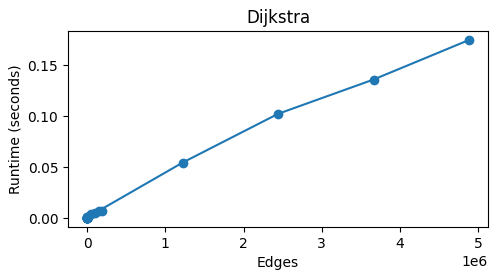
\includegraphics[scale=1]{dijk.png}{a}
        \caption{Dijkstra - Número de Arestas x Runtime}
\end{figure}

\begin{figure}[H]
    \centering
        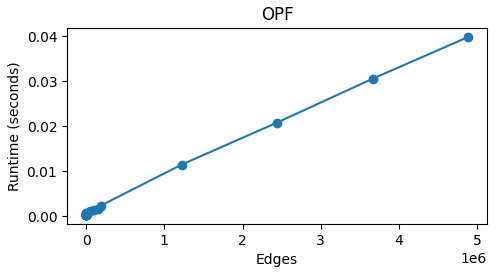
\includegraphics[scale=1]{opf.png}{b}
        \caption{Opf - Número de Arestas x Runtime}
\end{figure}
Percebe-se, que os graficos obtidos pelo dijkstra e OPF são razoavelmente semelhantes, além de serem, dentre os algoritmos analisados, os com menor tempo de execução.
\begin{figure}[H]
    \centering
        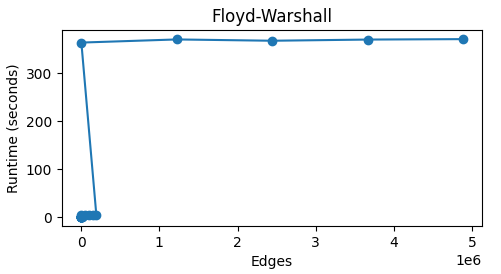
\includegraphics[scale=1]{floyd.png}{c}
        \caption{Floyd-Warshall - Número de Arestas x Runtime}
\end{figure}

\begin{figure}[H]
    \centering
        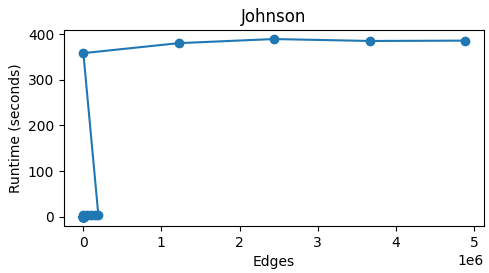
\includegraphics[scale=1]{john.png}{d}
        \caption{Johnson - Número de Arestas x Runtime}
\end{figure}

Percebe-se que tanto o johnson quanto o floyd-warshall se estabilizaram, e apesar do aumento de arestas, o tempo de execução se manteve em ambos os algoritmos.

\begin{figure}[H]
    \centering
        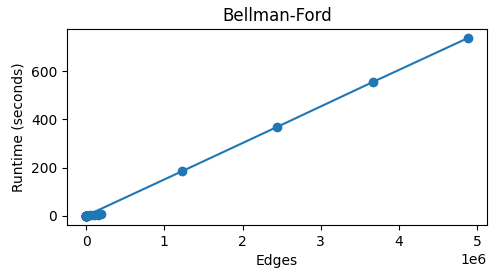
\includegraphics[scale=1]{bf.png}{e}
        \caption{Bellman-Ford - Número de Arestas x Runtime}
\end{figure}

Observa-se que o tempo de execução do bellman-ford cresceu junto com o número de arestas. Além disso, o bellman-ford foi algoritmo o com maior tempo de execução.

\begin{figure}[H]
    \centering
        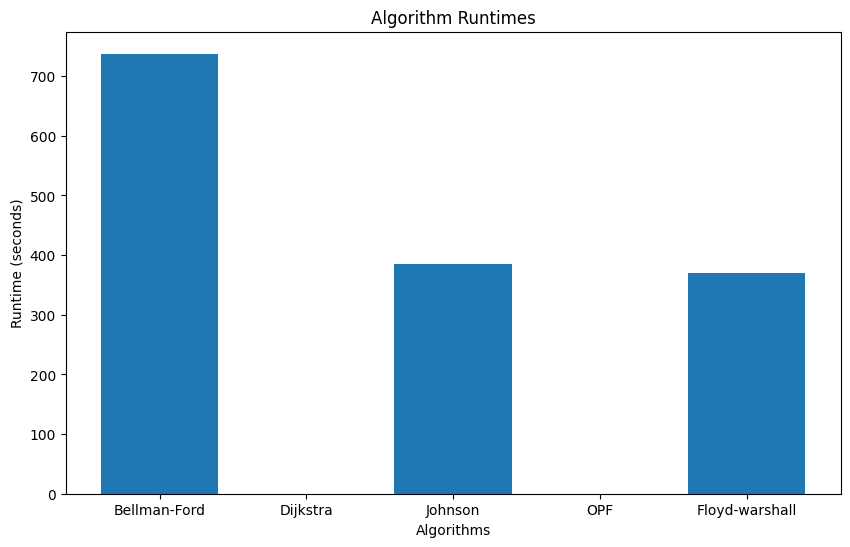
\includegraphics[scale=0.5]{allByTime_bars.png}{f}
        \caption{All algorithms - runtime (bars)}
\end{figure}

\begin{figure}[H]
    \centering
        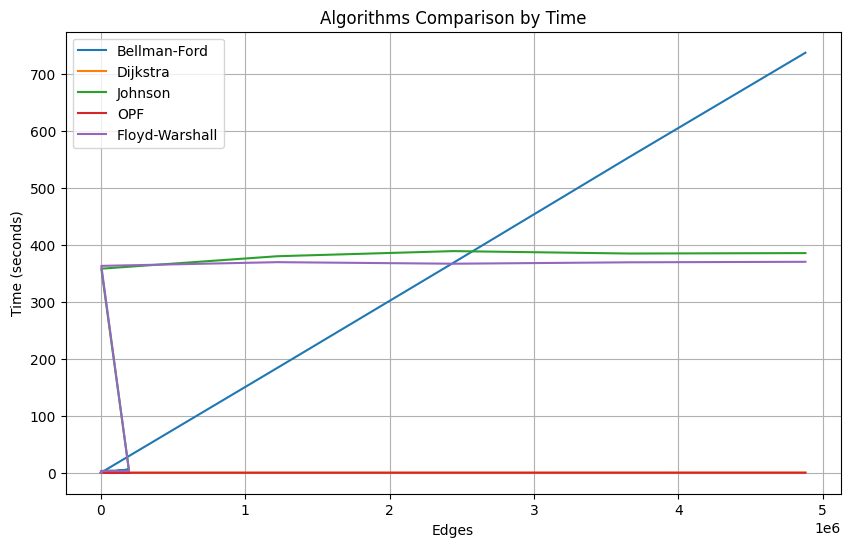
\includegraphics[scale=0.5]{allByTime_lines.png}{g}
        \caption{All algorithms - runtime (lines)}
\end{figure}

Ao comparar todos os algoritmos em um unico gráfico, é possível perceber com mais clareza que a diferença dos tempos de execução do Dijkstra e OPF para os outros algoritmos.

\begin{figure}[H]
    \centering
        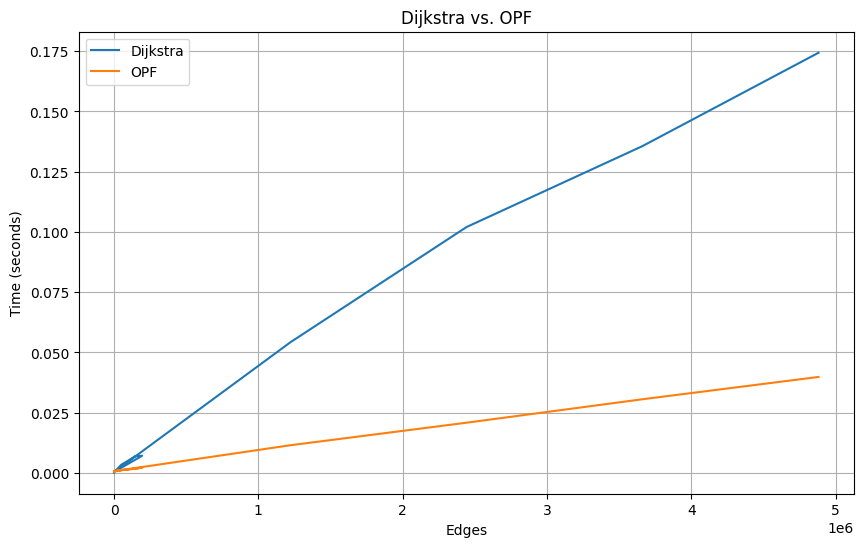
\includegraphics[scale=0.5]{opfxdijkstra.png}{h}
        \caption{Dijkstra x OPF - runtime}
\end{figure}


\begin{figure}[H]
    \centering
        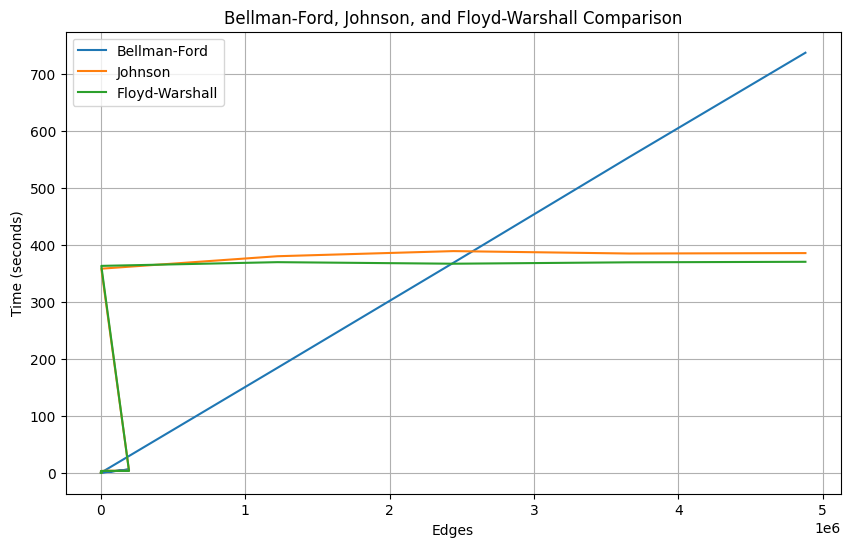
\includegraphics[scale=0.5]{belljohnsonfloyd.png}{i}
        \caption{Bellman-Ford x Floyd-Warshall x Johnson - runtime (lines)}
\end{figure}

Ao separar os gráficos em grupos, percebe-se como Bellman-Ford, Floyd-Warshall e Johnson estão em uma ordem de grandeza completamente diferente do Dijkstra e OPF

\section{Discussão dos resultados}

Na análise dos resultados obtidos, fica evidente que os cinco algoritmos - Dijkstra, OPF (\textit{Optimal Path Forest}), Algoritmo de Johnson, Bellman-Ford e Floyd-Warshall - apresentam diferentes desempenhos em relação ao tempo de execução, conforme ilustrado nos gráficos da seção anterior.

\subsection{Dijkstra e OPF}

Os gráficos revelam uma notável semelhança nos resultados entre os algoritmos Dijkstra e OPF. Além disso, destaca-se que ambos são os mais eficientes em termos de tempo de execução quando comparados aos demais algoritmos analisados. Esta similaridade não é surpreendente, dado que o OPF é uma variação do Dijkstra. Creio que a pequena diferença de desempenho observada pode ser atribuída à otimização do OPF, que, ao ajustar a condição de verificação, evita a entrada em determinadas condições, resultando em um tempo de execução algumas vezes mais rápido em comparação ao Dijkstra. Com essa abordagem, nem todos os vértices acabam sendo visitados, resultando em menos iterações do algoritmo. Isso contribui para um desempenho ligeiramente superior em comparação com o algoritmo de Dijkstra. A complexidade final de ambos os algoritmos foi de $O(v\log{}v)$, pois foi usada uma fila de prioridade para ordenação dos vértices.

\subsection{Johnson e Floyd-Warshall}

Os resultados para o Algoritmo de Johnson e Floyd-Warshall indicam uma estabilização do tempo de execução, mesmo com o aumento do número de arestas nos grafos. Essa estabilidade pode ser explicada pela natureza da implementação desses algoritmos, que dependem principalmente do número de vértices do grafo e não do número de arestas. Portanto, mesmo com variações nas condições do grafo, os tempos de execução permaneceram consistentes. A complexidade final do Floyd-Warshall foi $O(v^3)$, e a do algoritmo de johnson tambem foi de $O(v^3)$, mais especificamente $O(v^3 + v^2)$.

\subsection{Bellman-Ford}

Observa-se, por outro lado, que o tempo de execução do Bellman-Ford cresce proporcionalmente ao aumento do número de arestas nos grafos analisados. Isso se alinha com a expectativa, uma vez que a complexidade deste algoritmo depende do número de arestas. Notavelmente, o Bellman-Ford apresentou o maior tempo de execução entre os algoritmos considerados, o que destaca sua sensibilidade ao aumento da densidade de arestas nos grafos. A complexidade final do Bellman-Ford foi de $O(nm)$.

\section{Conclusão}

\subsection{Dijkstra e OPF}
No contexto do Dijkstra e OPF, a semelhança nos tempos de execução sugere que o OPF, como uma variação do Dijkstra, é capaz de preservar a eficiência fundamental deste último, enquanto em alguns casos demonstra vantagens decorrentes de otimizações específicas. Outro ponto a se dizer, é que apesar de servirem propósitos diferentes, é interessante perceber como algoritmos clássicos da literatura ajudam no desenvolvimento de novas soluções. Como Tanto o dijkstra quanto o OPF apresentam complexidade logarítmica, vale a pena utilizá-los nos mais diferentes cenários.

\subsection{Johnson e Floyd-Warshall}
Os Algoritmos de Johnson e Floyd-Warshall, por outro lado, exibiram estabilidade em seus tempos de execução, independentemente do aumento no número de arestas. Essa estabilidade, atribuída à dependência da complexidade em relação ao número de vértices, destaca a robustez desses algoritmos em cenários variáveis. O uso desses algoritmos compensa mais em grafos densos e com menos vértices.

\subsection{bellman-ford}
O Bellman-Ford, embora tenha se mostrado sensível ao crescimento do número de arestas, desempenhou um papel crucial ao revelar uma relação direta entre sua complexidade e a densidade de arestas nos grafos analisados. O Bellman-ford, como roda em cima das arestas, vale a pena ser utilizado em grafos esparços, ou seja, com menos arestas.

\subsection{Considerações Finais}
Em síntese, a escolha de um algoritmo específico deve ser pautada nas características particulares do problema em questão. Considerações como a preservação da eficiência, a estabilidade diante de variações e a sensibilidade a determinadas condições devem ser ponderadas.

\section{Referências}

\begin{enumerate}
    \item Antti Laaksonen. (2023). \textit{Competitive Programmer's Handbook}. Recuperado de: \url{https://cses.fi/book/book.pdf}
    
    \item \textit{Competitive Programming Algorithms}. Recuperado de: \url{https://cp-algorithms.com/}
    
    \item Alexandre Falcão. (Ano não especificado). \textit{Slides da disciplina MO443 - Processamento de Imagens}. Universidade Estadual de Campinas. Recuperado de: \url{https://ic.unicamp.br/~afalcao/mo443/slides-aula30.pdf}
    
    \item Reinhard Diestel. (Ano não especificado). \textit{Graph Theory}. Livro disponível em formato físico.
\end{enumerate}


\end{document}

